\documentclass[a4paper, 12pt]{article}

\usepackage[left=2cm,right=2cm,
top=2cm,bottom=2cm,bindingoffset=0cm]{geometry}

\usepackage[T2A]{fontenc}
\usepackage[utf8]{inputenc}
\usepackage{color}
\usepackage{graphicx}
\usepackage{caption}
\usepackage{listings}
\usepackage{subcaption}
\usepackage{tikz}
\usepackage{float}
\usepackage[english, russian]{babel}
\usepackage{amsmath,amsfonts,amssymb,amsthm,mathtools}
\usepackage{lscape}

\begin{document}
	\begin{center}
		\textbf{\textit{Задание}}
	\end{center}
	
	\begin{enumerate}
		\item Построить функции формы с помощью аппроксимации Лагранжа и Сирендипова семейства для квадратичного четырехугольного элемента 
		\item Вычислить производные от функций форм $\dfrac{\partial N_i}{\partial x}, \dfrac{\partial N_i}{\partial y}$
		\item Вычислить интеграл $\displaystyle \iint\limits_S \left(\dfrac{\partial N_i}{\partial x}\cdot \dfrac{\partial N_i}{\partial y}\right)\, dS$
	\end{enumerate}
	\begin{figure}[H]
		\centering
		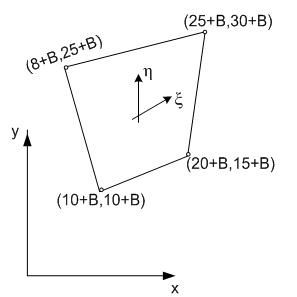
\includegraphics[width=0.3\linewidth]{task.png}
	\end{figure}

	\begin{center}
		\textbf{\textit{Решение}}
		
		\textbf{В = 7}
	\end{center}
	\begin{figure}[H]
		\centering
		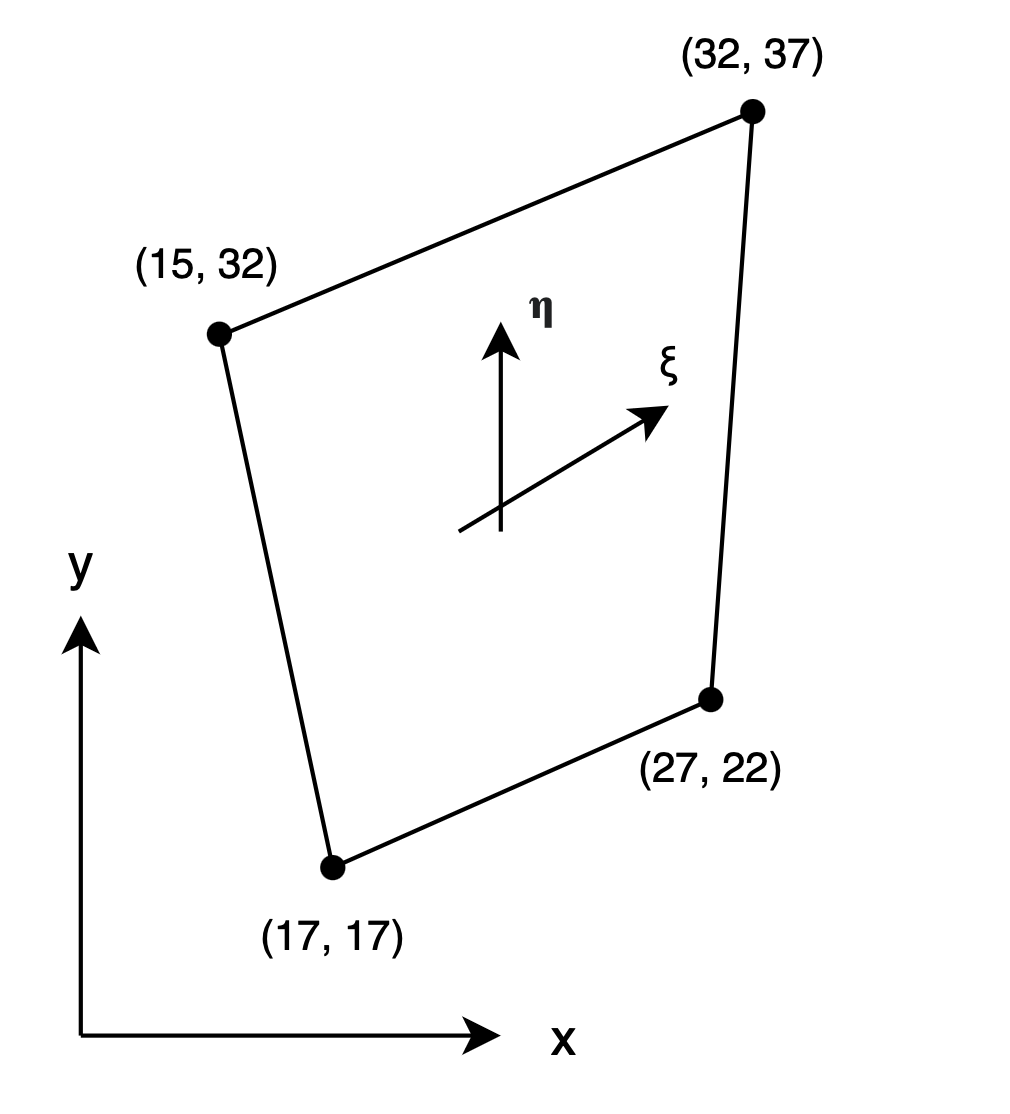
\includegraphics[width=0.3\linewidth]{mytask.png}
	\end{figure}
	
	В естественной системе координат:
	\begin{figure}[H]
		\centering
		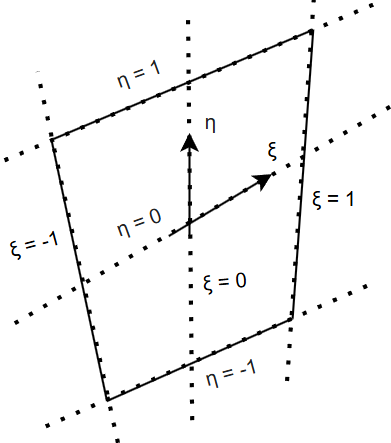
\includegraphics[width=0.3\linewidth]{ncs.png}
	\end{figure}
	\begin{center}
		\begin{tikzpicture}
			\draw(0,0) -- (4,0) -- (4,3) -- (0,3) -- cycle;
			\draw[->] (0,1.5) -- (5, 1.5) node[below right] {$\xi$};
			\draw[->] (2,0) -- (2,4) node[right] {$\eta$};
			\fill (0,0) circle(1.5pt);
			\fill (2,0) circle(1.5pt);
			\fill (4,0) circle(1.5pt);
			\fill (4,1.5) circle(1.5pt);
			\fill (0,1.5) circle(1.5pt);
			\fill (4,3) circle(1.5pt);
			\fill (2,3) circle(1.5pt);
			\fill (0,3) circle(1.5pt);
			\fill (2,1.5) circle(1.5pt);
			\node at (0,-0.5) {\footnotesize 1};
			\node at (2,-0.5) {\footnotesize 2};
			\node at (4,-0.5) {\footnotesize 3};
			\node at (4.25,1.75) {\footnotesize 4};
			\node at (4.25,3.25) {\footnotesize 5};
			\node at (1.75,3.25) {\footnotesize 6};
			\node at (-0.25,3.25) {\footnotesize 7};
			\node at (-0.25,1.75) {\footnotesize 8};
			\node at (2.25,1.75) {\footnotesize 0};
		\end{tikzpicture}
	\end{center}

	\begin{enumerate}
		\item Функции формы
		\begin{enumerate}
			\item Сирендипово семейство
			\[
				\varphi_2=\alpha_1+\alpha_2x+\alpha_3y+\alpha_4xy+\alpha_5x^2y+\alpha_6xy^2+\alpha_7x^2+\alpha_8y^2 
			\]

			Определим функции формы $N_{\beta}, \beta = \overline{1, 8}$ по формуле:
			\[
				N_{\beta} = \left[\prod_{j=1}^{4} F_j \right] 
				\left( a_{1\beta} + a_{2\beta}\xi + a_{3\beta}\eta \right), \quad
				F_k =
				\begin{cases} 
				f_k, & \text{если узел } \beta \notin \text{стороне } k, \\
				1, & \text{если узел } \beta \in \text{стороне } k,
				\end{cases}
			\]

			где $f_1 = (1 + \eta), f_2 = (1 - \xi), f_3 = (1 - \eta), f_4 = (1 + \xi)$.

			Вычислим функцию формы для элемента 1:
			\[
				N_1=(1-\eta)(1-\xi)(a_1+a_2\xi+a_3\eta) 
			\]
			\[ \begin{cases}
				N_1(\xi=0, \eta=-1)=0 \\
				N_1(\xi=-1, \eta=0) =0 \\
				N_1(\xi=-1, \eta=-1) = 1 \end{cases} \Rightarrow \begin{cases} N_1=2(a_1-a_3)=0 \\ N_1=2(a_1-a_2)=0 \\ N_1 = 4(a_1-a_2-a_3)=1  \end{cases}
			\]
			\[
			\Rightarrow a_1=a_2=a_3=-\frac{1}{4} 
			\]
			\[
				\Rightarrow N_1=-\frac{1}{4}(1-\eta)(1-\xi)(1+\xi+\eta) 
			\]

			Вычислим функцию формы для элемента 2:
			\[
			N_2=(\alpha_1+\alpha_2\xi+\alpha_3\eta+\alpha_4\xi\eta)(a_1+a_2\xi+a_3\eta)=(1+\xi)(1-\xi)(1-\eta)\cdot a \Rightarrow
			\]
			\[
				\Rightarrow 
				N_2(\xi=0, \eta=-1)=2a=1\Rightarrow a=\frac{1}{2} \Rightarrow N_2=\frac{1}{2}(1-\xi^2)(1-\eta)
			\]

			Аналогично для оставшихся элементов:
			\[
				N_3 = -\frac{1}{4}(1 + \xi)(1 - \eta)(1 - \xi + \eta)
			\]
			\[
				N_4 = \frac{1}{2}(1 + \xi)(1 - \eta^2)
			\]
			\[
				N_5 = -\frac{1}{4}(1 + \xi)(1 + \eta)(1 - \xi - \eta)
			\]
			\[
				N_6 = \frac{1}{2}(1 - \xi^2)(1 + \eta)
			\]
			\[
				N_7 = -\frac{1}{4}(1 - \xi)(1 + \eta)(1 + \xi - \eta)
			\]
			\[
				N_8 = \frac{1}{2}(1 - \xi)(1 - \eta^2)
			\]

			\item Лагранжево семейство
				\begin{center}
					\begin{tikzpicture}
						\draw(0,0) -- (4,0) -- (4,3) -- (0,3) -- cycle;
						\fill (0,0) circle(1.5pt);
						\fill (2,0) circle(1.5pt);
						\fill (4,0) circle(1.5pt);
						\fill (4,1.5) circle(1.5pt);
						\fill (0,1.5) circle(1.5pt);
						\fill (4,3) circle(1.5pt);
						\fill (2,3) circle(1.5pt);
						\fill (0,3) circle(1.5pt);
						\fill (2,1.5) circle(1.5pt);
						\node at (0,-0.5) {\footnotesize $\xi_i=-1$};
						\node at (2,-0.5) {\footnotesize $\xi_1=0$};
						\node at (4,-0.5) {\footnotesize $\xi_2=1$};
				
						\node at (-0.75,3.25) {\footnotesize $\eta_2=1$};
						\node at (-0.75,1.75) {\footnotesize $\eta_1=0$};
						\node at (-0.75,0.25) {\footnotesize $\eta_i=-1$};
				
						\draw(0.5,0.5) circle(8pt);
						\node at (0.5,0.5) {\footnotesize 1,1};
				
						\draw(0.5,1.75) circle(8pt);
						\node at (0.5,1.75) {\footnotesize 1,2};
					\end{tikzpicture}
				\end{center}

				Функция формы:
				\[
					N_{ij}=L_i^n(\xi)L_j^m(\eta)
				\]

				$L_i^n(\xi)L_j^m(\eta)$ - многочлены Лагранжа, $n,m$ - количество разбиений по $\xi, \eta$

				\[
					L_i^n(\xi)=\frac{(\xi-\xi_1)(\xi-\xi_2)\dots(\xi-\xi_n)}{(\xi_i-\xi_1)(\xi_i-\xi_2)\dots(\xi_i-\xi_n)}
				\]
				\[
					N_{ij}=L_i^2(\xi)L_j^2(\eta),\ i \neq 1,2
				\]
				\[
					L_i^2(\xi)=\frac{(\xi-\xi_1)(\xi-\xi_2)}{(\xi_i-\xi_1)(\xi_i-\xi_2)}
				\]
				\[
					N_1 = N_{11}=\frac{\xi\cdot(\xi-1)}{-1\cdot(-2)}\cdot \frac{\eta\cdot(\eta-1)}{-1\cdot(-2)}=\frac{1}{4}\cdot\xi\cdot\eta (\xi-1)(\eta-1)
				\]
				\[
					N_8 = N_{12}=\frac{\xi\cdot(\xi-1)}{2}\cdot \frac{(\eta+1)(\eta-1)}{1\cdot(-1)} = -\frac{1}{2} \xi(\xi - 1)(\eta^2 - 1)
				\]
				\[
					N_2 = \frac{(1 - \xi^2)\eta (\eta - 1)}{2}
				\]
				\[
					N_3 = \frac{\xi (\xi + 1)\eta (\eta - 1)}{4}
				\]
				\[
					N_4 = \frac{\xi (\xi + 1)(1 - \eta^2)}{2}
				\]
				\[
					N_5 = \frac{\xi (\xi + 1)\eta (\eta + 1)}{4}
				\]
				\[
					N_6 = \frac{(1 - \xi^2)\eta (\eta + 1)}{2}
				\]
				\[
					N_7 = \frac{\xi (\xi - 1) \eta (\eta + 1)}{4}
				\]
				\[
					N_0 = (\xi^2 - 1)(\eta^2 - 1)
				\]
			\end{enumerate}
		\newpage
		\item Вычислим производные от функций формы
		\[
			\begin{bmatrix}
				\frac{\partial N_{\beta}}{\partial \xi} \\
				\frac{\partial N_{\beta}}{\partial \eta}
			\end{bmatrix} = \begin{bmatrix}
			\frac{\partial x}{\partial \xi} & \frac{\partial x}{\partial \eta} \\
			\frac{\partial y}{\partial \xi} & \frac{\partial y}{\partial \eta}
			\end{bmatrix} \begin{bmatrix}
			\frac{\partial N_{\beta}}{\partial x} \\
			\frac{\partial N_{\beta}}{\partial y}
			\end{bmatrix} = 
			J \cdot \begin{bmatrix}
				\frac{\partial N_{\beta}}{\partial x} \\
				\frac{\partial N_{\beta}}{\partial y}
				\end{bmatrix}
			\Rightarrow \begin{bmatrix}
			\frac{\partial N_{\beta}}{\partial x} \\
			\frac{\partial N_{\beta}}{\partial y}
			\end{bmatrix}=J^{-1} \begin{bmatrix}
			\frac{\partial N_{\beta}}{\partial \xi} \\
			\frac{\partial N_{\beta}}{\partial \eta}
			\end{bmatrix}
		\]
		\[
			\begin{cases}
				x=R_1X_1+R_2X_2+R_3X_3+R_4X_4 \\
				y=R_1Y_1+R_2Y_2+R_3Y_3+R_4Y_4,
			\end{cases}
		\]

		где \(X_i, Y_i\) -- координаты вершин четырехугольника, \\
		$R_i$ -- линейные интерполяции:
		\[
			\begin{cases}
				R_1=\frac{1}{4}(1-\xi)(1-\eta) \\
				R_2=\frac{1}{4}(1+\xi)(1-\eta) \\
				R_3=\frac{1}{4}(1+\xi)(1+\eta) \\
				R_4=\frac{1}{4}(1-\xi)(1+\eta)
			\end{cases}
		\]

		Тогда:
		\[
			\begin{cases}
				x = \frac{17 \left(1 - \xi\right) \left(1 - \eta\right)}{4} + \frac{15 \left(1 - \xi\right) \left(\eta + 1\right)}{4} + \frac{27 \left(1 - \eta\right) \left(\xi + 1\right)}{4} + 8 \left(\xi + 1\right) \left(\eta + 1\right),\\
				y = \frac{17 \left(1 - \xi\right) \left(1 - \eta\right)}{4} + 8 \left(1 - \xi\right) \left(\eta + 1\right) + \frac{11 \left(1 - \eta\right) \left(\xi + 1\right)}{2} + \frac{37 \left(\xi + 1\right) \left(\eta + 1\right)}{4}.
			\end{cases}
		\]
		\[
			\begin{cases}
				x = \frac{7 \xi \eta}{4} + \frac{27 \xi}{4} + \frac{3 \eta}{4} + \frac{91}{4},\\
				y = \frac{5 \xi}{2} + \frac{15 \eta}{2} + 27.
			\end{cases}
		\]
		\[
			\frac{\partial x}{\partial \xi} = \frac{7 \eta}{4} + \frac{27}{4}, \quad \frac{\partial y}{\partial \xi} = \frac{5}{2}, \quad
			\frac{\partial x}{\partial \eta} = \frac{7 \xi}{4} + \frac{3}{4}, \quad \frac{\partial y}{\partial \eta} = \frac{15}{2}
		\]

		Матрица Якоби:
		\[
			J = 
			\left[\begin{matrix}\frac{7 \eta}{4} + \frac{27}{4} & \frac{5}{2}\\\frac{7 \xi}{4} + \frac{3}{4} & \frac{15}{2}\end{matrix}\right], \quad
			|J| = - \frac{35 \xi}{8} + \frac{105 \eta}{8} + \frac{195}{4}
		\]
		\[
			J^{-1} = \left[\begin{matrix}- \frac{12}{7\xi - 21\eta - 78} & \frac{4}{7\xi - 21\eta - 78}\\\frac{14\xi + 6}{35\xi - 105\eta - 390} & \frac{- 14\eta - 54}{35\xi - 105\eta - 390}\end{matrix}\right]
		\]
		\begin{enumerate}
			\item Сирендипово семейство
			\[
				\begin{bmatrix}
				\frac{\partial N_1}{\partial \xi} \\ 
				\frac{\partial N_1}{\partial \eta}
				\end{bmatrix}
				=
				-\frac{1}{4}
				\begin{bmatrix}
				(\eta - 1)(\eta + 2\xi) \\ 
				(2\eta + \xi)(\xi - 1)
				\end{bmatrix}
			\]

			\[
				\begin{bmatrix}
				\frac{\partial N_2}{\partial \xi} \\ 
				\frac{\partial N_2}{\partial \eta}
				\end{bmatrix}
				=
				\begin{bmatrix}
				\xi(\eta - 1) \\ 
				\frac{1}{2} - \frac{1}{2}\xi^2
				\end{bmatrix}
			\]

			\[
				\begin{bmatrix}
				\frac{\partial N_3}{\partial \xi} \\ 
				\frac{\partial N_3}{\partial \eta}
				\end{bmatrix}
				=
				\frac{1}{4}
				\begin{bmatrix}
				(\eta - 1)(\eta - 2\xi) \\ 
				(2\eta - \xi)(\xi + 1)
				\end{bmatrix}
			\]

			\[
				\begin{bmatrix}
				\frac{\partial N_4}{\partial \xi} \\ 
				\frac{\partial N_4}{\partial \eta}
				\end{bmatrix}
				=
				\begin{bmatrix}
				\frac{1}{2} - \frac{1}{2}\eta^2 \\ 
				-\eta(\xi + 1)
				\end{bmatrix}
			\]

			\[
				\begin{bmatrix}
				\frac{\partial N_5}{\partial \xi} \\ 
				\frac{\partial N_5}{\partial \eta}
				\end{bmatrix}
				=
				\frac{1}{4}
				\begin{bmatrix}
				(\eta + 1)(\eta + 2\xi) \\ 
				(2\eta + \xi)(\xi + 1)
				\end{bmatrix}
			\]

			\[
				\begin{bmatrix}
				\frac{\partial N_6}{\partial \xi} \\ 
				\frac{\partial N_6}{\partial \eta}
				\end{bmatrix}
				=
				\begin{bmatrix}
				-\xi(\eta + 1) \\ 
				\frac{1}{2} - \frac{1}{2}\xi^2
				\end{bmatrix}
			\]

			\[
				\begin{bmatrix}
				\frac{\partial N_7}{\partial \xi} \\ 
				\frac{\partial N_7}{\partial \eta}
				\end{bmatrix}
				=
				\frac{1}{4}
				\begin{bmatrix}
				(\eta + 1)(2\xi - \eta) \\ 
				(\xi - 2\eta)(\xi - 1)
				\end{bmatrix}
			\]

			\[
				\begin{bmatrix}
				\frac{\partial N_8}{\partial \xi} \\ 
				\frac{\partial N_8}{\partial \eta}
				\end{bmatrix}
				=
				\begin{bmatrix}
				\frac{1}{2}\eta^2 - \frac{1}{2} \\ 
				\eta(\xi - 1)
				\end{bmatrix}
			\]

			Итоговые производные:
			\[
				\begin{bmatrix}
				\frac{\partial N_1}{\partial x} \\ 
				\frac{\partial N_1}{\partial y}
				\end{bmatrix}
				=
				\left[\begin{matrix}\frac{\left(\xi - 1\right) \left(\xi + 2\eta\right) - 3 \left(2\xi +\eta\right) \left(\eta - 1\right)}{- 7\xi + 21\eta + 78}\\\frac{- \left(\xi - 1\right) \left(\xi + 2\eta\right) \left(7\eta + 27\right) + \left(2\xi +\eta\right) \left(7\xi + 3\right) \left(\eta - 1\right)}{10 \left(- 7\xi + 21\eta + 78\right)}\end{matrix}\right]
			\]

			\[
				\begin{bmatrix}
				\frac{\partial N_2}{\partial x} \\ 
				\frac{\partial N_2}{\partial y}
				\end{bmatrix}
				=
				\left[\begin{matrix}\frac{- 2\xi^{2} + 12\xi \left(\eta - 1\right) + 2.0}{- 7\xi + 21\eta + 78}\\\frac{- 2\xi \left(7\xi + 3\right) \left(\eta - 1\right) + \left(\xi^{2} - 1.0\right) \left(7\eta + 27\right)}{5 \left(- 7\xi + 21\eta + 78\right)}\end{matrix}\right]
			\]

			\[
				\begin{bmatrix}
				\frac{\partial N_3}{\partial x} \\ 
				\frac{\partial N_3}{\partial y}
				\end{bmatrix}
				=
				\left[\begin{matrix}\frac{\left(\xi + 1\right) \left(\xi - 2\eta\right) - 3 \left(2\xi -\eta\right) \left(\eta - 1\right)}{- 7\xi + 21\eta + 78}\\\frac{- \left(\xi + 1\right) \left(\xi - 2\eta\right) \left(7\eta + 27\right) + \left(2\xi -\eta\right) \left(7\xi + 3\right) \left(\eta - 1\right)}{10 \left(- 7\xi + 21\eta + 78\right)}\end{matrix}\right]
			\]

			\[
				\begin{bmatrix}
				\frac{\partial N_4}{\partial x} \\ 
				\frac{\partial N_4}{\partial y}
				\end{bmatrix}
				=
				\left[\begin{matrix}\frac{- 6\eta^{2} + 4\eta \left(\xi + 1\right) + 6.0}{- 7\xi + 21\eta + 78}\\\frac{- 2\eta \left(\xi + 1\right) \left(7\eta + 27\right) + \left(7\xi + 3\right) \left(\eta^{2} - 1.0\right)}{5 \left(- 7\xi + 21\eta + 78\right)}\end{matrix}\right]
			\]

			\[
				\begin{bmatrix}
				\frac{\partial N_5}{\partial x} \\ 
				\frac{\partial N_5}{\partial y}
				\end{bmatrix}
				=
				\left[\begin{matrix}\frac{- \left(\xi + 1\right) \left(\xi + 2\eta\right) + 3 \left(2\xi +\eta\right) \left(\eta + 1\right)}{- 7\xi + 21\eta + 78}\\\frac{\left(\xi + 1\right) \left(\xi + 2\eta\right) \left(7\eta + 27\right) - \left(2\xi +\eta\right) \left(7\xi + 3\right) \left(\eta + 1\right)}{10 \left(- 7\xi + 21\eta + 78\right)}\end{matrix}\right]
			\]

			\[
				\begin{bmatrix}
				\frac{\partial N_6}{\partial x} \\ 
				\frac{\partial N_6}{\partial y}
				\end{bmatrix}
				=
				\left[\begin{matrix}\frac{2\xi^{2} - 12\xi \left(\eta + 1\right) - 2.0}{- 7\xi + 21\eta + 78}\\\frac{2\xi \left(7\xi + 3\right) \left(\eta + 1\right) - \left(\xi^{2} - 1.0\right) \left(7\eta + 27\right)}{5 \left(- 7\xi + 21\eta + 78\right)}\end{matrix}\right]
			\]

			\[
				\begin{bmatrix}
				\frac{\partial N_7}{\partial x} \\ 
				\frac{\partial N_7}{\partial y}
				\end{bmatrix}
				=
				\left[\begin{matrix}\frac{- \left(\xi - 1\right) \left(\xi - 2\eta\right) + 3 \left(2\xi -\eta\right) \left(\eta + 1\right)}{- 7\xi + 21\eta + 78}\\\frac{\left(\xi - 1\right) \left(\xi - 2\eta\right) \left(7\eta + 27\right) - \left(2\xi -\eta\right) \left(7\xi + 3\right) \left(\eta + 1\right)}{10 \left(- 7\xi + 21\eta + 78\right)}\end{matrix}\right]
			\]

			\[
				\begin{bmatrix}
				\frac{\partial N_8}{\partial x} \\ 
				\frac{\partial N_8}{\partial y}
				\end{bmatrix}
				=
				\left[\begin{matrix}\frac{6\eta^{2} - 4\eta \left(\xi - 1\right) - 6.0}{- 7\xi + 21\eta + 78}\\\frac{2\eta \left(\xi - 1\right) \left(7\eta + 27\right) - \left(7\xi + 3\right) \left(\eta^{2} - 1.0\right)}{5 \left(- 7\xi + 21\eta + 78\right)}\end{matrix}\right]
			\]
			\item Лагранжево семейство
			\[
				\begin{bmatrix}
				\frac{\partial N_1}{\partial \xi} \\ 
				\frac{\partial N_1}{\partial \eta}
				\end{bmatrix}
				=
				\frac{1}{4}
				\begin{bmatrix}
				\eta (2\xi - 1)(\eta - 1) \\ 
				(\xi - 1)(2\eta - 1)\xi
				\end{bmatrix}
			\]

			\[
				\begin{bmatrix}
				\frac{\partial N_2}{\partial \xi} \\ 
				\frac{\partial N_2}{\partial \eta}
				\end{bmatrix}
				=
				\begin{bmatrix}
				\xi \eta (1 - \eta) \\ 
				\left(\eta - \frac{1}{2}\right)(1 - \xi^2)
				\end{bmatrix}
			\]

			\[
				\begin{bmatrix}
				\frac{\partial N_3}{\partial \xi} \\ 
				\frac{\partial N_3}{\partial \eta}
				\end{bmatrix}
				=
				\frac{1}{4}
				\begin{bmatrix}
				\eta (2\xi + 1)(\eta - 1) \\ 
				(\xi + 1)(2\eta - 1)\xi
				\end{bmatrix}
			\]

			\[
				\begin{bmatrix}
				\frac{\partial N_4}{\partial \xi} \\ 
				\frac{\partial N_4}{\partial \eta}
				\end{bmatrix}
				=
				\begin{bmatrix}
				\left(\xi + \frac{1}{2}\right)(1 - \eta^2) \\ 
				-\eta(\xi + 1)\xi
				\end{bmatrix}
			\]

			\[
				\begin{bmatrix}
				\frac{\partial N_5}{\partial \xi} \\ 
				\frac{\partial N_5}{\partial \eta}
				\end{bmatrix}
				=
				\frac{1}{4}
				\begin{bmatrix}
				(\eta + 1)(2\xi + 1)\eta \\ 
				(2\eta + 1)(\xi + 1)\xi
				\end{bmatrix}
			\]

			\[
				\begin{bmatrix}
				\frac{\partial N_6}{\partial \xi} \\ 
				\frac{\partial N_6}{\partial \eta}
				\end{bmatrix}
				=
				\begin{bmatrix}
				-\xi \eta (\eta + 1) \\ 
				\left(\eta + \frac{1}{2}\right)(1 - \xi^2)
				\end{bmatrix}
			\]

			\[
				\begin{bmatrix}
				\frac{\partial N_7}{\partial \xi} \\ 
				\frac{\partial N_7}{\partial \eta}
				\end{bmatrix}
				=
				\frac{1}{4}
				\begin{bmatrix}
				(\eta + 1)\eta(2\xi - 1) \\ 
				(2\eta + 1)(\xi - 1)\xi
				\end{bmatrix}
			\]

			\[
				\begin{bmatrix}
				\frac{\partial N_8}{\partial \xi} \\ 
				\frac{\partial N_8}{\partial \eta}
				\end{bmatrix}
				=
				\begin{bmatrix}
				\left(\xi - \frac{1}{2}\right)(1 - \eta^2) \\ 
				\xi \eta (1 - \xi)
				\end{bmatrix}
			\]

			\[
				\begin{bmatrix}
				\frac{\partial N_0}{\partial \xi} \\ 
				\frac{\partial N_0}{\partial \eta}
				\end{bmatrix}
				=
				\begin{bmatrix}
				2\xi (\eta^2 - 1) \\ 
				2 \eta (\xi^2 - 1)
				\end{bmatrix}
			\]

			Итоговые производные:
			\[
				\begin{bmatrix}
				\frac{\partial N_1}{\partial x} \\ 
				\frac{\partial N_1}{\partial y}
				\end{bmatrix}
				=
				\left[\begin{matrix}\frac{-\xi \left(\xi - 1\right) \left(2\eta - 1\right) + 3\eta \left(2\xi - 1\right) \left(\eta - 1\right)}{- 7\xi + 21\eta + 78}\\\frac{x \left(\xi - 1\right) \left(2\eta - 1\right) \left(7\eta + 27\right) -\eta \left(2\xi - 1\right) \left(7\xi + 3\right) \left(\eta - 1\right)}{10 \left(- 7\xi + 21\eta + 78\right)}\end{matrix}\right]
			\]

			\[
				\begin{bmatrix}
				\frac{\partial N_2}{\partial x} \\ 
				\frac{\partial N_2}{\partial y}
				\end{bmatrix}
				=
				\left[\begin{matrix}\frac{4 \left(- 3\xi\eta \left(\eta - 1\right) + \left(\xi^{2} - 1\right) \left(\eta - 0.5\right)\right)}{- 7\xi + 21\eta + 78}\\\frac{2 \left(\xi\eta \left(7\xi + 3\right) \left(\eta - 1\right) - \left(\xi^{2} - 1\right) \left(\eta - 0.5\right) \left(7\eta + 27\right)\right)}{5 \left(- 7\xi + 21\eta + 78\right)}\end{matrix}\right]
			\]

			\[
				\begin{bmatrix}
				\frac{\partial N_3}{\partial x} \\ 
				\frac{\partial N_3}{\partial y}
				\end{bmatrix}
				=
				\left[\begin{matrix}\frac{-\xi \left(\xi + 1\right) \left(2\eta - 1\right) + 3\eta \left(2\xi + 1\right) \left(\eta - 1\right)}{- 7\xi + 21\eta + 78}\\\frac{x \left(\xi + 1\right) \left(2\eta - 1\right) \left(7\eta + 27\right) -\eta \left(2\xi + 1\right) \left(7\xi + 3\right) \left(\eta - 1\right)}{10 \left(- 7\xi + 21\eta + 78\right)}\end{matrix}\right]
			\]

			\[
				\begin{bmatrix}
				\frac{\partial N_4}{\partial x} \\ 
				\frac{\partial N_4}{\partial y}
				\end{bmatrix}
				=
				\left[\begin{matrix}\frac{4 \left(\xi\eta \left(\xi + 1\right) - 3 \left(\xi + 0.5\right) \left(\eta^{2} - 1\right)\right)}{- 7\xi + 21\eta + 78}\\\frac{2 \left(-\xi\eta \left(\xi + 1\right) \left(7\eta + 27\right) + \left(\xi + 0.5\right) \left(7\xi + 3\right) \left(\eta^{2} - 1\right)\right)}{5 \left(- 7\xi + 21\eta + 78\right)}\end{matrix}\right]
			\]

			\[
				\begin{bmatrix}
				\frac{\partial N_5}{\partial x} \\ 
				\frac{\partial N_5}{\partial y}
				\end{bmatrix}
				=
				\left[\begin{matrix}\frac{-\xi \left(\xi + 1\right) \left(2\eta + 1\right) + 3\eta \left(2\xi + 1\right) \left(\eta + 1\right)}{- 7\xi + 21\eta + 78}\\\frac{x \left(\xi + 1\right) \left(2\eta + 1\right) \left(7\eta + 27\right) -\eta \left(2\xi + 1\right) \left(7\xi + 3\right) \left(\eta + 1\right)}{10 \left(- 7\xi + 21\eta + 78\right)}\end{matrix}\right]
			\]

			\[
				\begin{bmatrix}
				\frac{\partial N_6}{\partial x} \\ 
				\frac{\partial N_6}{\partial y}
				\end{bmatrix}
				=
				\left[\begin{matrix}\frac{4 \left(- 3\xi\eta \left(\eta + 1\right) + \left(\xi^{2} - 1\right) \left(\eta + 0.5\right)\right)}{- 7\xi + 21\eta + 78}\\\frac{2 \left(\xi\eta \left(7\xi + 3\right) \left(\eta + 1\right) - \left(\xi^{2} - 1\right) \left(\eta + 0.5\right) \left(7\eta + 27\right)\right)}{5 \left(- 7\xi + 21\eta + 78\right)}\end{matrix}\right]
			\]

			\[
				\begin{bmatrix}
				\frac{\partial N_7}{\partial x} \\ 
				\frac{\partial N_7}{\partial y}
				\end{bmatrix}
				=
				\left[\begin{matrix}\frac{-\xi \left(\xi - 1\right) \left(2\eta + 1\right) + 3\eta \left(2\xi - 1\right) \left(\eta + 1\right)}{- 7\xi + 21\eta + 78}\\\frac{x \left(\xi - 1\right) \left(2\eta + 1\right) \left(7\eta + 27\right) -\eta \left(2\xi - 1\right) \left(7\xi + 3\right) \left(\eta + 1\right)}{10 \left(- 7\xi + 21\eta + 78\right)}\end{matrix}\right]
			\]

			\[
				\begin{bmatrix}
				\frac{\partial N_8}{\partial x} \\ 
				\frac{\partial N_8}{\partial y}
				\end{bmatrix}
				=
				\left[\begin{matrix}\frac{4 \left(\xi\eta \left(\xi - 1\right) - 3 \left(\xi - 0.5\right) \left(\eta^{2} - 1\right)\right)}{- 7\xi + 21\eta + 78}\\\frac{2 \left(-\xi\eta \left(\xi - 1\right) \left(7\eta + 27\right) + \left(\xi - 0.5\right) \left(7\xi + 3\right) \left(\eta^{2} - 1\right)\right)}{5 \left(- 7\xi + 21\eta + 78\right)}\end{matrix}\right]
			\]

			\[
				\begin{bmatrix}
				\frac{\partial N_0}{\partial x} \\ 
				\frac{\partial N_0}{\partial y}
				\end{bmatrix}
				=
				\left[\begin{matrix}\frac{8 \left(3\xi \left(\eta^{2} - 1\right) -\eta \left(\xi^{2} - 1\right)\right)}{- 7\xi + 21\eta + 78}\\\frac{4 \left(-\xi \left(7\xi + 3\right) \left(\eta^{2} - 1\right) +\eta \left(\xi^{2} - 1\right) \left(7\eta + 27\right)\right)}{5 \left(- 7\xi + 21\eta + 78\right)}\end{matrix}\right]
			\]
		\end{enumerate}
		\newpage
		\item Вычислим интеграл $\displaystyle \iint\limits_S \left(\dfrac{\partial N_i}{\partial x}\cdot \dfrac{\partial N_i}{\partial y}\right)\, dS$
		\[
			Z = \int_{-1}^{1} \int_{-1}^{1} f(\xi, \eta) \, d\eta d\xi = \sum_{i=1}^n \sum_{j=1}^n H_i H_j f(\xi_i, \eta_j)
		\]
		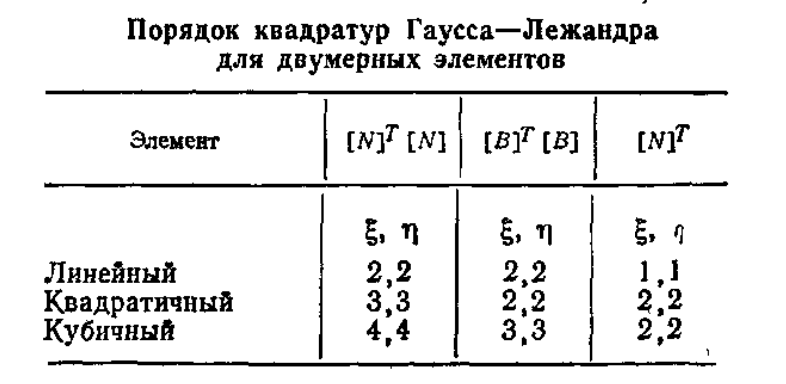
\includegraphics[scale=0.3]{int1.png}
		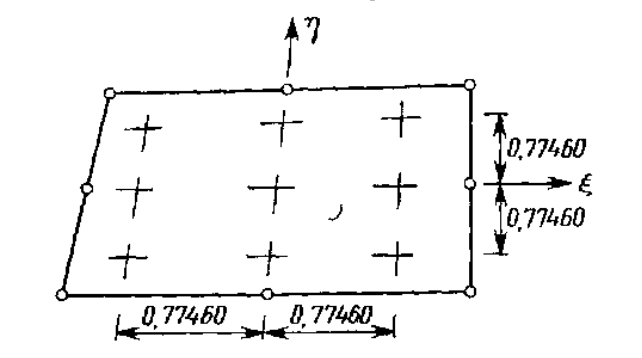
\includegraphics[scale=0.3]{int2.png}
		\begin{center}
			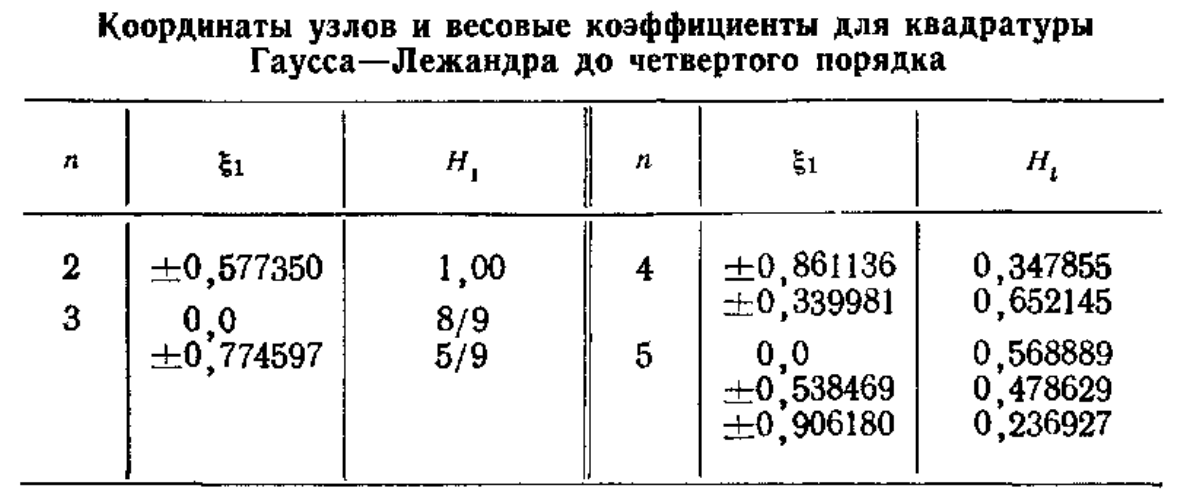
\includegraphics[scale=0.3]{int3.png}
		\end{center}
		Для Сирендипова семейства получаем \(Z = 0.3296\), для Лагранжева \(0.5737\).

	\end{enumerate}
	
\end{document}